\chapter{Testing and Experimental Results}
\justify

Product development has been completed for the project, and as a result, all functionalities have been thoroughly tested. This chapter presents a comprehensive overview of the features tested, providing screenshots and photographs of hardware to illustrate the outcome of the built systems.

\section{Testing Methodology}

The testing phase involved various methodologies to ensure the functionality, performance, and reliability of Open-source Intelligence Data Mining System and  "Call One" caller ID  android app. The following testing methods were employed:

\begin{enumerate}[label=\roman*.]
    \item \textbf{Unit Testing:} Testing individual modules and components to verify their correctness and functionality. Jest an nodejs module is used to test the components of the the android app and call one app's backend. The example test results is depicted in figure \ref{fig:JestTesting} .

    \item \textbf{Testing and Debugging}: Used flipper to test the state of the application in different phase and checking shared preferences as shown in the figure \ref{fig: Testing and Debugging} and \ref{fig:Flipper Debugging Tool}.
 
    \item \textbf{Performance Testing:} Assessing the app's performance under various load conditions. Used FlatList to render contacts and call logs to implove the performance. As showing in the Figure \ref{fig: Performance Testing} the performance score is 91 and on average it is rendering 57 frames per second.

\end{enumerate}

\begin{figure}
    \centering
    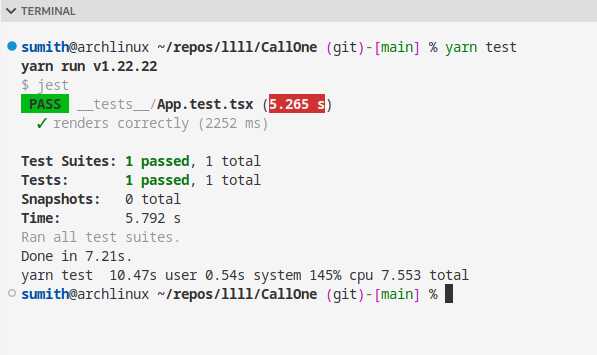
\includegraphics[width=1\linewidth]{Media//Chapter 6/jest.png}
    \caption{Jest Testing}
    \label{fig:JestTesting}
\end{figure}

\begin{figure}
    \centering
    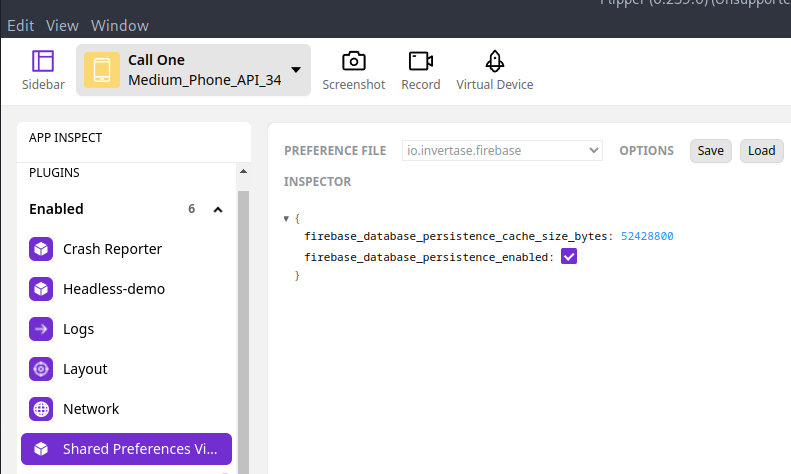
\includegraphics[width=1\linewidth]{Media//Chapter 6/sharedprefs.png}
    \caption{Testing and Debugging}
    \label{fig: Testing and Debugging}
\end{figure}

\begin{figure}
    \centering
    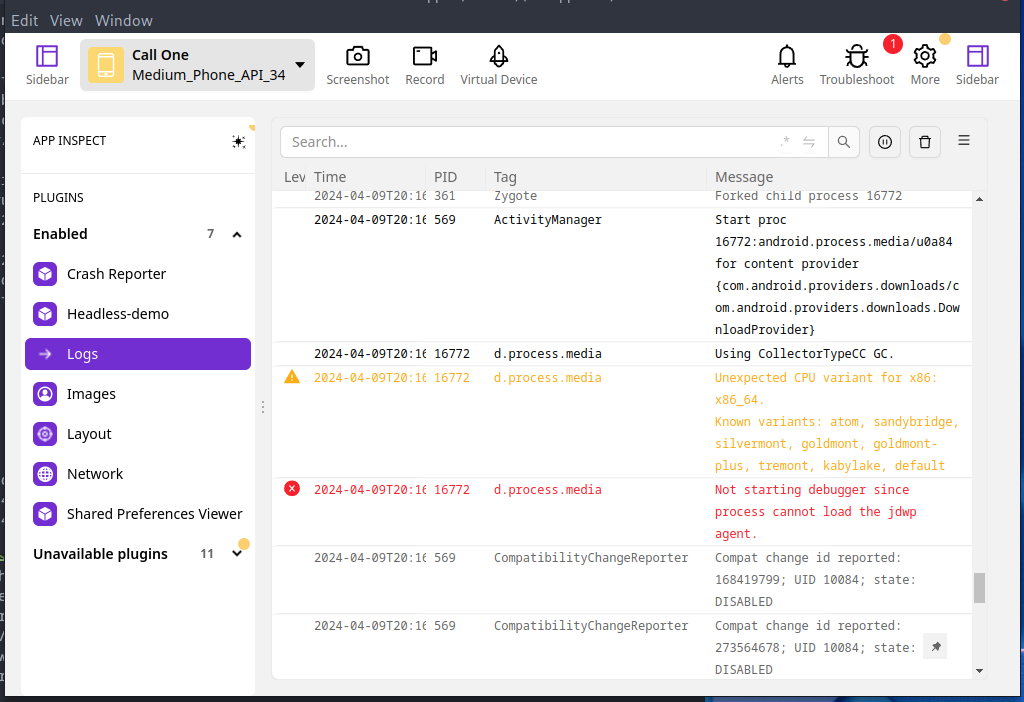
\includegraphics[width=1\linewidth]{Media//Chapter 6/flipper.png}
    \caption{Flipper Debugging}
    \label{fig:Flipper Debugging Tool}
\end{figure}

\begin{figure}
    \centering
    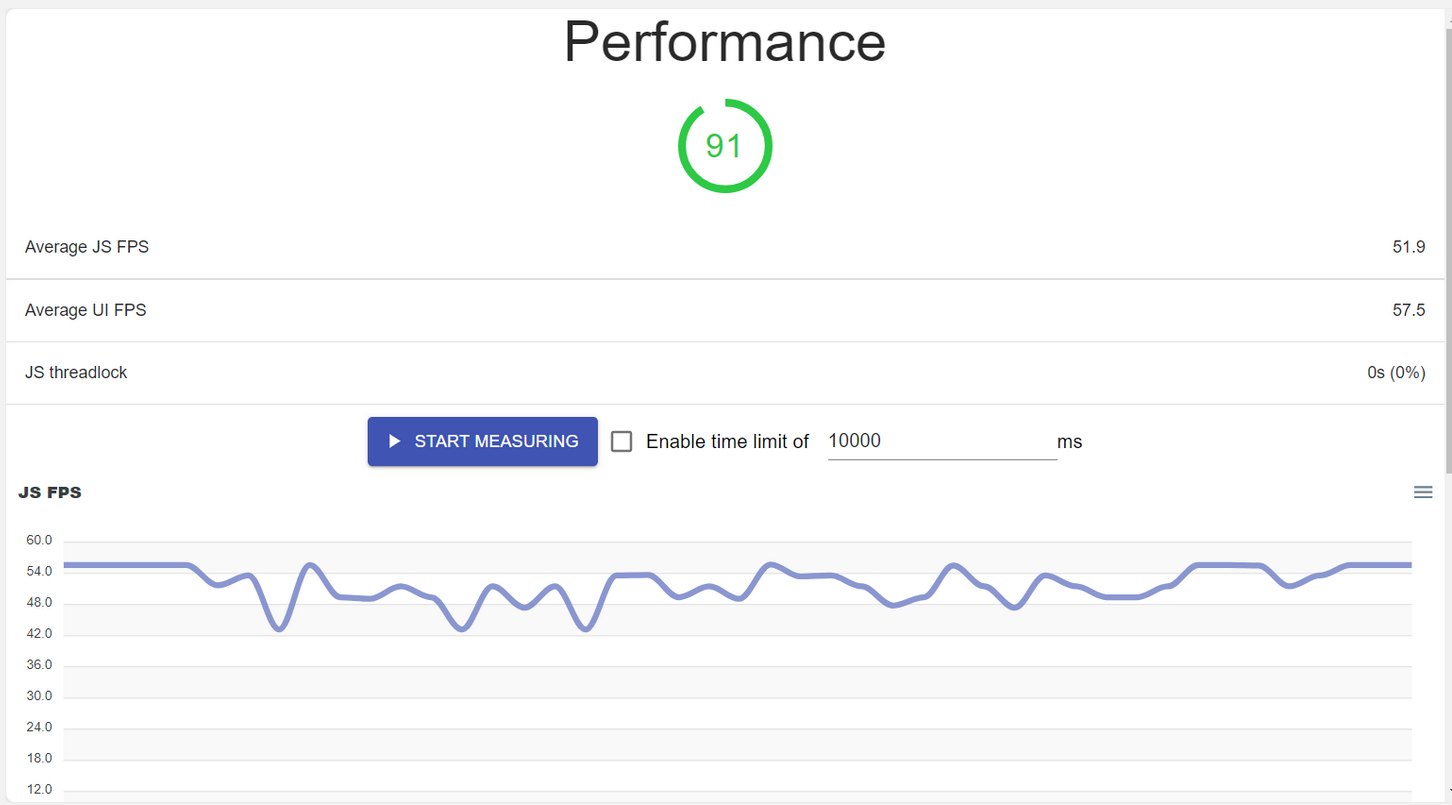
\includegraphics[width=1\linewidth]{Media//Chapter 6/performance.png}
    \caption{Performance Testing}
    \label{fig: Performance Testing}
\end{figure}

\section{Experimental Results}

The experimental results of the testing phase demonstrated the following outcomes:

\begin{enumerate}[label=\roman*.]
    \item \textbf{Functionalities Verified:} All functionalities of the "Call One" app were verified and found to be working as expected.
    
    \item \textbf{Performance Optimization:} Performance testing revealed that the app performs optimally under various load conditions, ensuring smooth user experience.
    
\end{enumerate}

After conducting the tests, all the test cases had been passed, the bugs had been fixed, and it's ready to be released. The flow of testing and fixing the bugs is depicted in the figure \ref{fig:Testing}.


\begin{figure}
    \centering
    \includegraphics[width=1\linewidth]{Media/Chapter 6/diagram_testing.png}
    \caption{Testing}
    \label{fig:Testing}
\end{figure}


\section{Screenshots and Photographs}

Visual representations of the tested features, user interface, and hardware setup are provided below for reference and illustration.

\begin{figure}
    \centering
    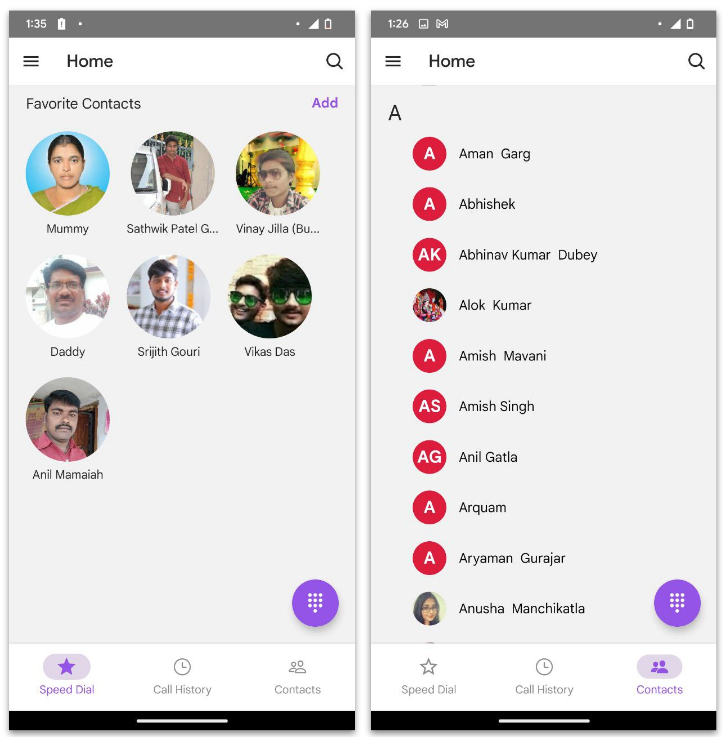
\includegraphics[width=1\linewidth]{Media//demo.png}
    \caption{Demo}
    \label{fig:App demo image}
\end{figure}


\begin{figure}
    \centering
    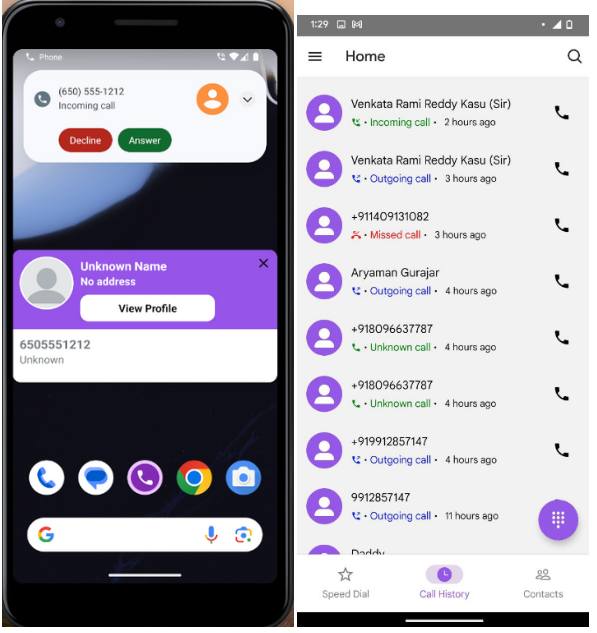
\includegraphics[width=1\linewidth]{Media/demo2.png}
    \caption{Demo 2}
    \label{fig:App Start}
\end{figure}